\section{Trace d'exécution}
Ci-dessous l'exécution du programme sur trois hôtes. Au niveau de l'affichage, il est à noter qu'à chaque fois que la file est modifiée, son contenu est affiché à l'aide de \textbf{print\_messages\_linked\_list()}.

\begin{figure}[h!]
    \centering
    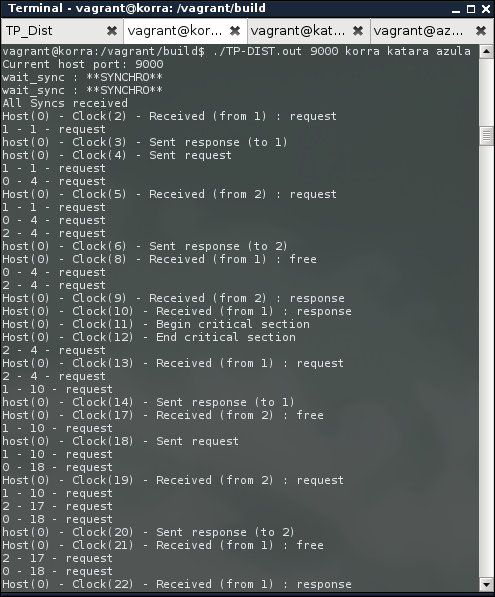
\includegraphics[width=0.7\textwidth]{screenshots/h0_korra.png}
    \caption{host 0}
\end{figure}%

\begin{figure}[h!]
    \centering
    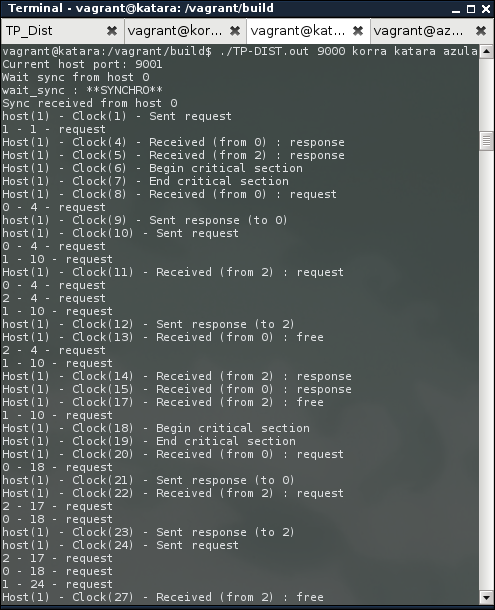
\includegraphics[width=0.7\textwidth]{screenshots/h1_katara.png}
    \caption{host 1}
\end{figure}

\begin{figure}[h!]
    \centering
    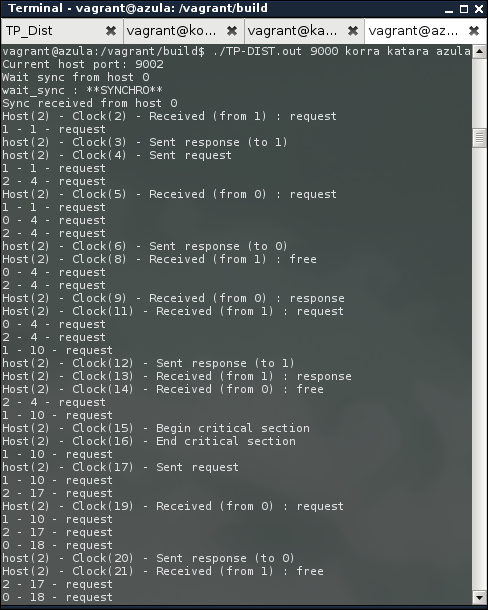
\includegraphics[width=0.7\textwidth]{screenshots/h2_azula.png}
    \caption{host 2}
\end{figure}
